\documentclass[12pt]{article}
\usepackage[english]{babel}
\usepackage{amsmath}
\usepackage{graphicx}
\usepackage{textcomp}
\usepackage{siunitx}
\usepackage{parskip}
\usepackage[colorinlistoftodos]{todonotes}
\usepackage{csquotes}
\usepackage{float}
\usepackage{algpseudocode}
\usepackage{algorithm}
\usepackage{url}
\usepackage{hyperref}
\usepackage{xcolor}
\usepackage{tikz}
\usepackage{geometry}
\usepackage{seqsplit}
\geometry{verbose,tmargin=2cm,bmargin=2cm,lmargin=3cm,rmargin=3cm}
\usepackage[backend=biber,style=alphabetic,sorting=ynt]{biblatex}
\addbibresource{cites.bib}

\setlength {\marginparwidth }{2cm}
\begin{document}
	
	% \begin{titlepage}
		
	% 	\newcommand{\HRule}{\rule{\linewidth}{0.5mm}}
	% 	\centering
		
	% 	\textsc{\LARGE University of New South Wales}\\[1.5cm]
	% 	\includegraphics[scale=0.8]{logo.PNG}\\[1cm]
	% 	\textsc{\Large COMP4121 - Project Report}\\[0.5cm] 
		
	% 	\HRule \\[0.4cm]
	% 	{ \huge \bfseries Application of Fast Fourier Transformation on Image Processing}\\[0.4cm] 
	% 	\HRule \\[1.5cm]
		
	
	% 	\begin{center}
	% 		\begin{tabular}{ c      c } 
	% 			Haoming Wang & z5270005
	% 		\end{tabular}
	% 	\end{center}
		
	% 	\vfill
	% 	{\large \today}\\[1cm] 
	% 	\vfill 
		
	% \end{titlepage}
	
	\begin{abstract}
		DFT (Discrete Fourier Transformation) is a mathematics concept that converts a finite sequence of equally spaced samples of a function into same length sequence of equally spaced samples which will result in a complex valued function of frequency, on top of the result of transformation, operations can be performed, such as, to eliminate noise in signal wave, compression of the image.
		DFT can be also represented as a matrix multiplication and use the matrix multiplication to optimise the performance of computation. 
		
		Whereas FFT (Fast Fourier Transformation) is the computing algorithm that implements DFT to boost the computation performance that allows the data set to be larger and optimise the time complexity from $O(n^2)$ into $O(nlogn)$.
		In this report, FFT will be implemented from scratch in Rust language and explain how is it be used in image processing.
	\end{abstract}
	
	\pagebreak
	
	\setcounter{page}{1}
	\thispagestyle{empty}
	\tableofcontents
	\pagebreak
	\setcounter{page}{1}
	
	
	\pagebreak
	\section{Introduction}
		
		\subsection{Fourier Series} \label{subsec:1.1}
			
			To have more in depth discussion in FFT, one very important tool will be using is Fourier series, it is defined as 
			\begin{center}
			\centering
				$f(x) = \sum_{n=0}^{\infty}(a_{n}\cos nx + b_{n}\sin nx) $ 
			\end{center}
			where $n$ is the frequency of samples and $a_{n}, b_{n}, c_{n}$ are the coefficients that need to be solved. It can be written in a complex form $\sum_{-\infty}^{\infty} = c_{n} e^{inx}$, the latter function will be very useful when DFT and FFT comes in where it has unity of roots and complex number inclusion. The target is to find $a_{n}, b_{n}, c_{n}$, the key is orthogonality, which is inner product (dot product). Written in integral is $\int_{-\pi}^{\pi}(\cos nx)(\cos kx) dx = 0$. It is in order to divide functions into frequencies which can give a diagram that shows the harmonics. The lower harmonic ie, $\cos 2x$ have a smoother curve and the high harmonics like $\cos 100x$ have a quicker changes in the function.  
			
		\subsection{Solve of Coefficients in the Fourier Series}
			By the definition in \ref{subsec:1.1}, where $\int_{-\pi}^{\pi}(\cos nx)(\cos kx) dx = 0$. By multiply a $\cos kx$ on the both sides. 
			
			\begin{center}
				\centering
				$\int_{-\pi}^{\pi} f(x) \cos kx dx = \int_{-\pi}^{\pi} (\sum_{n=0}^{\infty} a_{n} \cos nx \sin nx) \cos kx dx$
			\end{center}
		
			if $n = k$, $\implies \int_{-\pi}^{\pi} (\cos kx)^{2} dx$, because only $n = k$ would survive in the process, other terms would be zeros in the integration. Then result of the integration is $a_{k}\pi$. Thus, $a_{k} = \frac{1}{\pi} \int_{-\pi}^{\pi} \cos kn dx$, similarly, $b_{k} = \frac{1}{\pi} \int_{-\pi}^{\pi} \sin kn dx$.
			The use of solving the coefficient is used to know what is the harmonics of sinusoidal and cosinusodial functions, a signal - image or sound wave, are consist of infinite many cosine and sine functions stack together, that is the reason the graph of frequency versus time is a wavy shaped segment.
			
		
		\subsection{Proof of Orthogonality as Change of Basis}
			
			To understand Fourier Series and Fourier Transformation, an important property is orthogonality, because it is an orthogonal transformation in essence. The given function is denoted as $e^{i \frac{2\pi}{n}} = \cos \frac{2\pi}{n} + i\sin \frac{2\pi}{n}$ and can be represented as $\omega_{n}$, because of it is a root of unity, there is a property that $\omega_{n}^{n} = 1$, as in \ref{subsec:1.1}, to proof the orthogonality, a basis should be introduced that is 
			
			\begin{center}
				\centering
		
				$F = \{f_{0}, f_{1}, ..., f_{n -1}\}$, where $f_{k} = \{(\omega_{n}^{k})^{0}, (\omega_{n}^{k})^{1}, ..., (\omega_{n}^{k})^{n-1}\}$. 
			\end{center}
			Assume that $k \neq m$, $\langle f_{n},f_{m}\rangle = \sum_{i=0}^{n-1}(\omega_{n}^{ki})\overline{(\omega_{n}^{mi})}$ should be zero, the sum of inner product of $\omega_{n}$ power of $k$ and power of $i$ and conjugate of $\omega_{n}$ power of $m$ and power of $i$ since the definition of inner product of complex numbers. By expanding the conjugate, 
			\begin{center}
			\centering
				$\sum_{i=0}^{n-1}(\omega_{n}^{k})^{ki}(\omega_{n}^{k})^{-mi} = \sum_{i=0}^{n-1}(\omega_{n}^{k})^{(k-m)i}, k \neq m$ and let $q = \omega_{n}^{k - m}$, else $q=1$. 
			\end{center}
			Where $q$ represent the geometry progression ratio, in another words, how many of $q$'s stacking in the sum every time in the inner product, so that,
			
			\begin{center}
			\centering
				$\sum_{i=0}^{n-1}q^{i} = \frac{1-q^{n}}{1-q}$
				
			\end{center}
			
			by substitute $q$ in the inner product, can get,
			\begin{center}
				\centering
				$\langle f_{k}, f_{m} \rangle = \frac{1-(\omega_{n}^{k-m})^{n}}{1-\omega_{n}^{k-m}} = \frac{1-(\omega_{n}^{n})^{k-m}}{1-\omega_{n}^{k-m}} = \frac{1-(1)^{k-m}}{1-\omega_{n}^{k-m}}$ 
				
				(this can be referred to the beginning of the proof where $\omega_{n}^{n}$)
				
				$\implies \frac{1-1}{1-\omega_{n}^{k-m}} = 0$
				
				Q.E.D
			\end{center}
		
	
	\section{Matrix Representation}
		By introduce a complex matrix, $F_{n}$, where,
		
		\begin{center}
			\centering
			
			$
			\begin{bmatrix}
			1 & 1 & 1 & \cdots & 1 \\
			1 & \omega & \omega^{2} & \cdots & \omega^{n-1} \\
			\vdots & \vdots & \vdots & \ddots & \vdots \\
			1 & \omega^{n-1} & \omega^{2(n-1)} & \cdots & \omega^{(n-1)^{2}}
			\end{bmatrix}
			$
			
			
		\end{center}
		let $V$ denote the Vandermonde matrix, let $\vec{A}$ denote the vector of coefficients $(a_{0}, a_{1}, \cdots, a_{n-1})$ and vector $\vec{y} = (y_{0}, y_{1}, \cdots, y_{n-1})$, where $V_{jk} = x_{j}^{k}$ for $x_{j} = e^{\frac{2\pi ji}{n}}$ and the transform from coefficient to discrete samples is $V\vec{A} = \vec{y}$.
		
		Therefore the transformation can be like a transform on a unit circle, it needs $n$ numbers of complex numbers, divide a unit circle into $n$ pieces,
		
		\begin{center}
			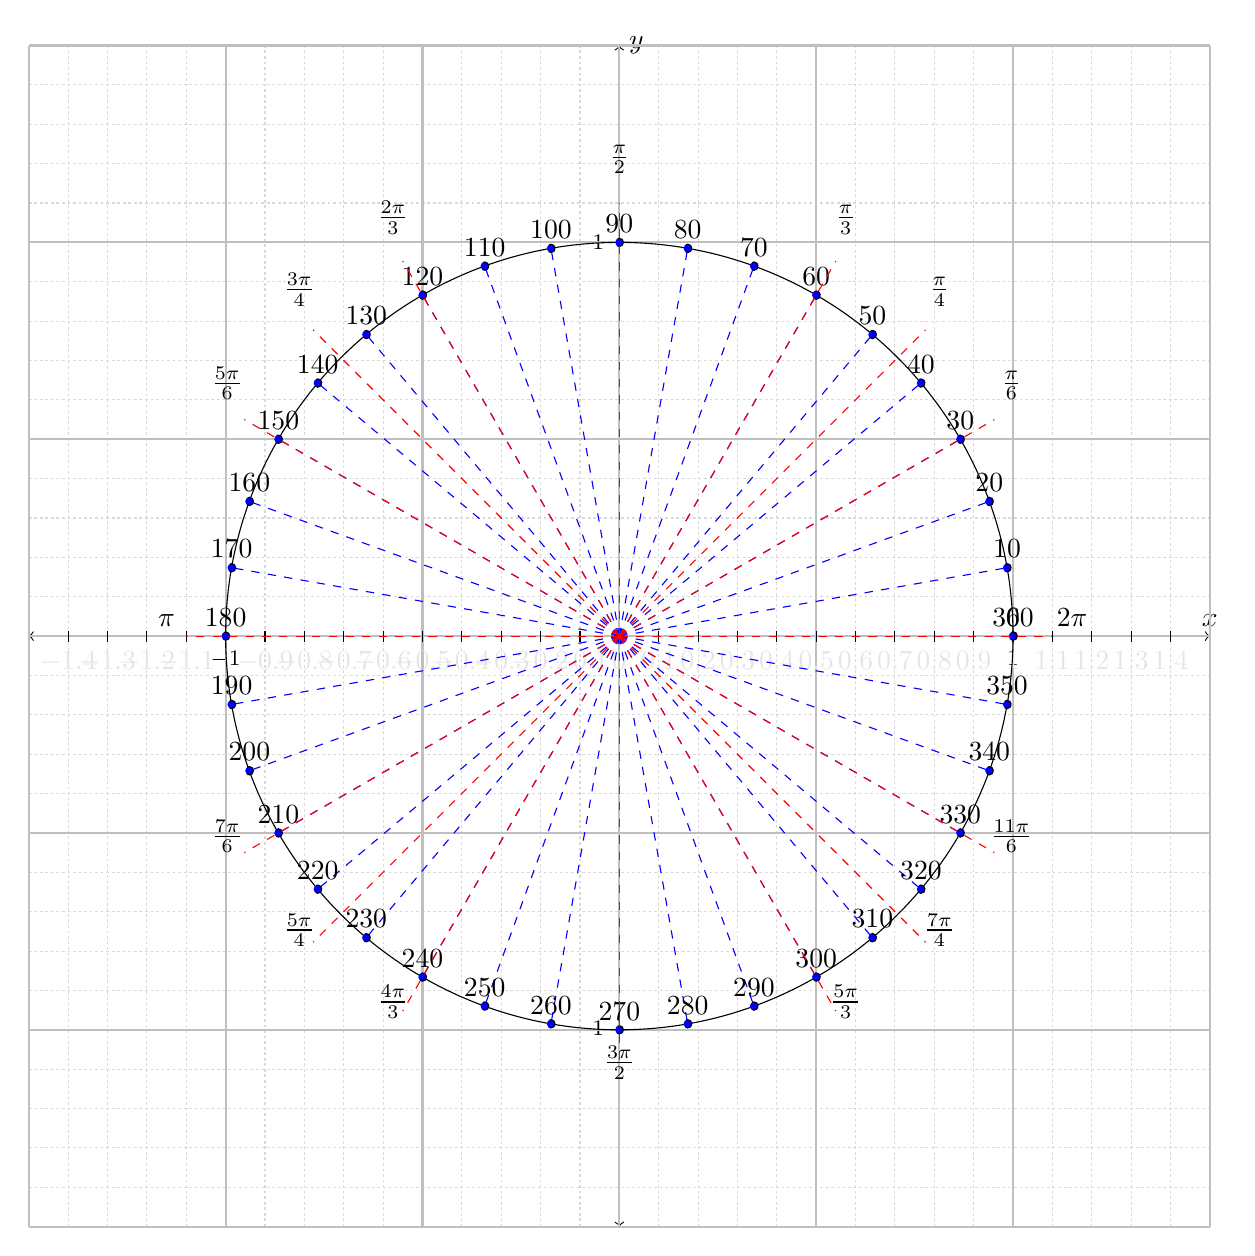
\begin{tikzpicture}[x=5cm,y=5cm]
			\draw[<->] (-1.5,0)--(1.5,0)node[above]{$x$};
			\draw[<->] (0,-1.5)--(0,1.5)node[right]{$y$};
			
			\foreach \x in {-1,1}
			\draw[shift={(\x,0)}](0pt,2pt)--(0,-2pt)node[below]{\footnotesize $\x$};
			
			\foreach \y in {-1,1}
			\draw[shift={(0,\y)}](2pt,0pt)--(-2pt,0pt)node[left]{\footnotesize $\y$};
			\draw [color=gray!30,dash pattern=on 1pt off 1pt, xstep=0.1,ystep=0.1] (-1.5,-1.5) grid (1.5,1.5);
			\draw[thick,gray!50,xstep=0.5,ystep=0.5](-1.5,-1.5) grid (1.5,1.5);
			\foreach \x in {-1.4,-1.3,-1.2,-1.1,-0.9,-0.8,-0.7,-0.6,-0.5,-0.4,-0.3,-0.2,-0.1,0,0.1,0.2,0.3,0.4,0.5,0.6,0.7,0.8,0.9,1,1.1,1.2,1.3,1.4}
			\draw(\x,2pt)--(\x,-2pt)node[below,gray!20]{$\x$};
			%\draw[shift={(\x,0)}](0pt,2pt)--(0,-2pt)node[color=gray,rotate=90]{\footnotesize $\x$};
			
			%\foreach \y in {-1.4,-1.3,-1.2,-1.1,-0.9,-0.8,-0.7,-0.6,-0.5,-0.4,-0.3,-0.2,-0.1,0,0.1,0.2,0.3,0.4,0.5,0.6,0.7,0.8,0.9,1,1.1,1.2,1.3,1.4}
			%    \draw(\y,0)node[below,gray!30]{$\y$};
			%\draw[shift={(0,\y)}](2pt,0pt)--(-2pt,0pt)node[color=gray,left]{\footnotesize $\y$};
			
			\draw (0,0) circle (1);
			
			\foreach \x in {0,10,...,360}
			\draw[dashed,color=blue] (0,0)--(\x:1);
			\foreach \x in {0,10,...,360}
			\draw [dashed,fill=blue] (\x:1) circle (1.5pt)node[sloped,above]{$\x$};
			
			\foreach \x/\xtext in {             
				30/\frac{\pi}{6},             
				45/\frac{\pi}{4},             
				60/\frac{\pi}{3},             
				90/\frac{\pi}{2},             
				120/\frac{2\pi}{3},             
				135/\frac{3\pi}{4},             
				150/\frac{5\pi}{6},             
				180/\pi,             
				210/\frac{7\pi}{6},             
				225/\frac{5\pi}{4},             
				240/\frac{4\pi}{3},             
				270/\frac{3\pi}{2},             
				300/\frac{5\pi}{3},             
				315/\frac{7\pi}{4},             
				330/\frac{11\pi}{6},             
				360/2\pi
			}                 
			\draw (\x:5.75cm) node[above] {$\xtext$};
			\foreach \x in {0,30,...,360}
			\draw[dashed,color=red] (0,0)--(\x:5.5cm);
			\foreach \x in {0,45,...,360}
			\draw[dashed,color=red] (0,0)--(\x:5.5cm);
			\end{tikzpicture}
		\end{center}
		from coordinate (1, 0), the geometry ratio of $\omega_{n}^{k}$, can produce a vector and input the vector into polynomial representation, which is a linear mapping then can produces a series of special complex coordinate, which is the result of the transformation.
	
	
	\section{Complexity Analysis of FFT}
		In the matrix view, the transform is conducted in reducing the size of matrix, for example a $64 \times 64$ matrix, to reduce the multiplications of the matrix.
		\begin{center}
			\centering
			
			$
			\begin{bmatrix}
			F_{64}
			\end{bmatrix}
			=
			\begin{bmatrix}
			I & D\\
			I & -D
			\end{bmatrix}
			\begin{bmatrix}
			F_{32} & 0\\
			0 & F_{32}
			\end{bmatrix}
			\begin{bmatrix}
			P
			\end{bmatrix}
			$
			
			
		\end{center}
		where $P$ is the permutation matrix and $D$ is the diagonal matrix 
		\begin{center}
			\centering
				$D = \begin{bmatrix}
				1 & 0 & \cdots & 0\\
				0 & \omega & \cdots & 0\\
				\vdots & \vdots & \ddots & \vdots \\
				0 & 0 & \cdots & \omega^{31}
				\end{bmatrix}$
		\end{center}
		
		by reducing the size of matrix, next step is as following,
		\begin{center}
			\centering
			
			$
			\begin{bmatrix}
			F_{64}
			\end{bmatrix}
			=
			\begin{bmatrix}
			I & D\\
			I & -D
			\end{bmatrix}
			\begin{bmatrix}
				\begin{bmatrix}
				I & D\\
				I & -D
				\end{bmatrix} & 0\\
				0 & \begin{bmatrix}
				I & D\\
				I & -D
				\end{bmatrix}
			\end{bmatrix}
			\begin{bmatrix}
				\begin{bmatrix}
				F_{16} & 0\\
				0 & F_{16}
				\end{bmatrix} & \begin{bmatrix}
				0 & 0\\
				0 & 0
				\end{bmatrix} \\
				\begin{bmatrix}
				0 & 0\\
				0 & 0
				\end{bmatrix} & \begin{bmatrix}
				F_{16} & 0\\
				0 & F_{16}
				\end{bmatrix}
			\end{bmatrix}
			\begin{bmatrix}
			P & 0\\
			0 & P
			\end{bmatrix}
			\begin{bmatrix}
				P
			\end{bmatrix}
			$
			
			
		\end{center}
		In the end the whole chain of matrix multiplication will be divided into $F_{2}$. Thus the performance boost of matrix multiplication is from $O(n^{2})$ to $O(n\log n)$, where $n$ is the size of the matrix and $n = 2^{x}, x \in \Re$.
		
		Without using FFT to do the matrix multiplication, the efficiency is low, a $64 \times 64$ matrix need $64^{2}$ operations, which is 4096 times of multiplication, but in the FFT performance boost, the multiplication times reduced to approximately 115 times, which saves $\frac{1}{35}$ of the computation time.
		
	\section{Implementation}
		\subsection{FFT}
			FFT (Fast Fourier Transformation) pseudo code where in complex field to define $\omega$, n-th root of unity.
			
			\begin{algorithm}[H]
				\caption{Fast Fourier Transformation} \label{alg:cap}
				\begin{algorithmic}
					\Require $A$ - Reference of array of value with length $n$. $flag$ - Boolean value (flag) indicates FFT or iFFT.
					
					\Ensure $n = 2^{x}, x \in \Re$
					
					\Procedure{FFT}{$A$, $flag$}
					
					\If{n = 1}
						
						return $A$
					\EndIf
					
					\State $a_{odd} \gets$ array of $\frac{n}{2}$ values.
					\State $a_{even} \gets$ array of $\frac{n}{2}$ values.
					
					\For{$idx$ in $0..n$ step by 2}
					
						$a_{odd}[\frac{idx}{2}] \gets A[idx]$
						
						$a_{even}[\frac{idx}{2}] \gets A[idx + 1]$
					\EndFor
					
					FFT($a_{odd}$, $flag$)
					
					FFT($a_{even}$, $flag$)
					
					\If{$flag$ is True}
					
					\State $x \gets 1$
					\Else 
					
					\State $x \gets -1$
					\EndIf
					
					\State $\omega_{n} = \cos \frac{2\pi}{n} + x \times \sin \frac{2\pi}{n}i$
					
					\State $\omega_{0} = 1 + 0i$
					
					\For{$idx$ in 0..$\frac{n}{2}$}
						
						$A[idx] = a_{odd}[idx] + \omega_{0} \times a_{even}[idx] $
						
						$A[idx + \frac{n}{2}] = a_{odd}[i] - \omega_{0} \times a_{even}[idx]$
						
						$\omega_{0} = \omega_{0} \times \omega_{n}$
					\EndFor
					\EndProcedure
					
					
				\end{algorithmic}
			\end{algorithm}
			FFT is a classic divide and conquer algorithm, the required argument is an array, denoted as A (reference or pointer) and a flag to indicate if it is an inverse fft. It initially set up a base condition for the recursion when length of array is 1, return. Then, if the length is not 1, create 2 separate arrays which is the half length of array A, one is for even index and one is for odd index. Do a for loop, fill the even and odd array by filling the corresponding value at specific index from array A. Next is to recursively parse even array and odd array in the procedure again over again, by continuously splitting the array into even and odd parts, for example an array $[1, 2, 3, 4, 5, 6, 7, 8]$, will be firstly split into an even array of $[1, 3, 5, 7]$ and odd array $[2, 4, 5, 8]$, note that the 'even' or 'odd' is determined by the index not the value itself. It will recursively partition the array until it only left 1 element in the recursion tree. Next step is to determine if the procedure is called for FFT ot IFFT, if represent FFT algorithm on a unit circle, then FFT is rotation from a coordinate to another coordinate, e.g. rotate the coordinate $(\frac{\sqrt{3}}{2}, \frac{1}{2})$ which is the $\ang{30}$, to $(0, 1)$, which is $\ang{90}$. IFFT is to rotate $(0, 1)$ back t0 $(\frac{\sqrt{3}}{2}, \frac{1}{2})$. Therefore it is the invert direction operation, adding a negative sign in front of the omega construction is the solution. First is to construct the $\omega_{n}$, which is by defined formula, $\cos \frac{2\pi}{n} + x \times \sin \frac{2\pi}{n}i$. Second, make $\omega_{0}$, $1 + 0i$, in a loop, update array A according to the index from 0 to half of array length in both odd and even parts. Finally, update the $\omega_{0}$ by multiply $\omega_{n}$. 
		
		\subsection{FFT 2D}
		
			FFT 2D is the 2 dimensional version of FFT, which in the image processing, it includes a width and a height. In traditional FFT, it is widely used on boosting the performance of polynomial multiplication, the integer array piped into FFT procedural will produce an array of transformed values which is in complex form. Where in form of equation, the 2 dimensional FFT is represented as following,
			
			\begin{center}
				\centering
				
				$F(u, v) = \sum_{m=0}^{m-1} \sum_{n=0}^{n-1} f(x,y) e^{-i2\pi (\frac{ux}{m} + \frac{vy}{n})}$
			\end{center}
		
			In this image processing algorithm, the way to do the FFT on pixels is to first read the RGB values from the picture, pictures can be represented as a matrix with each cell has RGB value, for instance, a $3 \times 3$ pixels picture can be represent like following,
			
			\begin{center}
				\centering
				\[
				\begin{bmatrix}
					(244, 255, 231) & (211, 212, 100) & (23, 32, 76)\\
					(231, 98, 78) & (21, 11, 90) & (98, 74, 32)\\
					(21, 22, 09) & (32, 21, 55) & (44, 23, 99)
				\end{bmatrix}
				\]
			\end{center}
		
			each cell is a tuple of RGB value, by reading the matrix, and decompose each tuple, get all R, G, B values individually, pipe into the original 1 dimensional FFT then after the transform, assemble the values together and store or display it (in this project, is to display the result of the transformation).
		\subsection{Digital Watermarking}
			Digital watermarking is used in many real life situations, a very close example is picture watermarking. However, simple watermark on a picture sometimes can ruin the overall quality of the image, or can be cropped out by image editing tools. The digital watermark is embedding an image A into another image B, but the image A is hidden in image B, because of the robustness of image objects, for instance, JPEG, any attack including cropping, contamination of the image would not affect the final watermark, and by using IFFT, or a tool that can load frequency graph of IFFT, for example MATLAB, watermark can be easily checked if the image is altered. It can be used in steganography, secret encryption and file (image or sound) transformation integrity check.
			
			Additionally, in the source code, in fft\_2d function, the ratio of opacity can be adjusted, currently the ratio between watermark and original picture is 2:8, but it can be adjusted according to user's preference. The higher watermark ratio is, the more unclear original picture will be, and a small shadow of the watermark can be shown in the middle of the image.
			
			% \begin{figure}[H]
			% 	\caption{Ratio in Implementation of FFT-2D}
			% 	\centering
			% 	\includegraphics[scale=0.8]{fft2dimpl.JPG}\\[1cm]
			% \end{figure}
		
		
			% \begin{figure}[H]
			% 	\caption{Final Effect and Test Run on CSE}
			% 	\centering
			% 	\includegraphics[scale=0.8]{testruncse.JPG}\\[1cm]
			% \end{figure}
		
			
			% \begin{figure}[H]
			% 	\caption{Sample Picture Used}
			% 	\centering
			% 	\includegraphics[scale=0.8]{samplepic.JPG}\\[1cm]
			% \end{figure}
		
			
			% \begin{figure}[H]
			% 	\caption{Sample Watermark Used}
			% 	\centering
			% 	
\includegraphics[scale=0.8]{watermark.JPG}\\[1cm]
			% \end{figure}
			
	
		\subsection{Setup and Build Information}
		
				The implementation of the algorithm is built and tested on \href{https://www.debian.org/}{Debian} and \href{https://archlinux.org/}{Arch} based systems. The essential build toolchain for the project is \href{https://rustup.rs/}{rustup}, which contains the Rust package manager `Cargo' and `rustc' the \href{https://www.rust-lang.org/}{Rust} compiler.
				
				Visit this \href{https://rustup.rs/}{\textit{\textbf{link}}} to install rustup.
				
				Otherwise, detailed build and run information is included in README.md.
				
		\subsection{Parts Can Be Improved}
			\begin{itemize}
				\item The implementation is mainly using CPU for image computation, the performance is relatively inefficient, it can be boost by GPU calculation, for instance, CUDA.
				
				\item Parameters can be added to the program so that it can provide user a better way to customise their preferences. For example, a parameter to resize the image, a parameter can choose the opacity of the watermark.
			\end{itemize}
		\pagebreak
	\section{References}
 		\begin{itemize}
 			\item Yang, S., \& Ignjatovic, A. (2022). The Discrete Fourier Transform, Discrete Cosine Transform, Convolution
 			and their Applications. Retrieved from:
 			\seqsplit{http://www.cse.unsw.edu.au/~cs4121/lectures\_2022/week7/DFT\_DCT\_CONV\_short.pdf}.
 			
 			\item MIT OpenCourseWare. (2016). 3. Divide \& Conquer: FFT. Retrieved from: \seqsplit{https://www.youtube.com/watch?v=iTMn0Kt18tg}.
 			
 			\item MIT OpenCourseWare. (2005). 26. Complex Matrices; Fast Fourier Transform. Retrieved from: \seqsplit{https://www.youtube.com/watch?v=M0Sa8fLOajA}.
 			
 			\item Uwaterloo, cs487 (n.d.) FFT Algorithm. Retrieved from: \seqsplit{https://cs.uwaterloo.ca/~kogeddes/cs487/LectureMaterials/Chapter\_4\_Materials/FFTalgorithm.pdf}.
 			
 			\item Schuster, P. (2021, March 17). Frequency Spectrum Analysis with FFT in Rust (library spectrum-analyzer). PHIPS BLOG. Retrieved from: \seqsplit{https://phip1611.de/blog/frequency-spectrum-analysis-with-fft-in-rust/}
 			
 			\item How to Interpret FFT results - complex DFT, frequency bins and FFTShift. (2015, November 16). GaussianWaves. Retrieved from: \seqsplit{https://www.gaussianwaves.com/2015/11/interpreting-fft-results-complex-dft-frequency-bins-and-fftshift/}
 			

 		\end{itemize}
	
\end{document}